\section{La fase de simulación}
\label{sec:Dataset}
Para lograr entrenar un modelo de Inteligencia Artificial que recree el movimiento de una tela se requiere de un dataset que represente el comportamiento de esta. En este apartado se explicará el proceso de obtención de datos, comenzando con qué tipo de simulación se elige para el estudio, continuando con las características o parámetros que mejor definen la tela y finalizando con la recogida de valores y creación del dataset a emplear en el entrenamiento. Todos los datos son generados de forma interna, creándose a partir de simulaciones de telas grabadas en Unity, por lo que se explicarán los componentes en la escena que permiten llevar esto a cabo.  % alguna especificacion a declarar? tipo necesitamos que nuestros datos sean de tal forma %
\subsection{La simulación}
\label{subsec:sim}
 La simulación base que se emplea para entrenar y ajustar los modelos se lleva a cabo en un escenario formado por un plano-tela de 25 vértices con la parte superior fija en el espacio y una esfera que colisiona con la tela para generar movimiento en ella.  \newline

\begin{figure}[H]
    \centering
    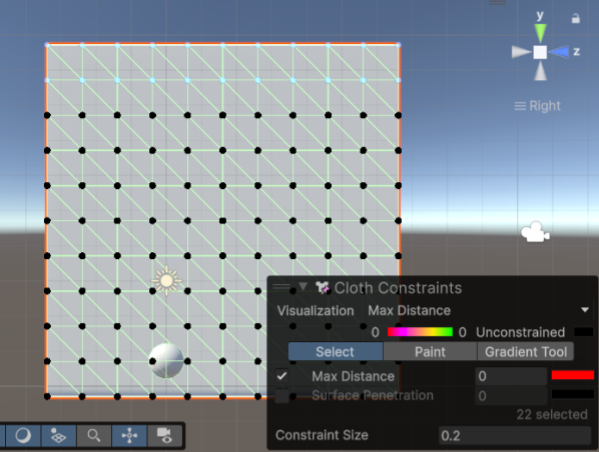
\includegraphics[width=0.5\textwidth]{Imagenes/Bmap/maxDistance.png}
    \caption{Malla de 25 vértices con parte superior fija.}
    \label{fig:maxDistance}
\end{figure}

El movimiento de la bola que colisiona con la tela está descrito por un componente \textit{BallMovement}. Este puede ser automático o generado a través de entrada con el teclado. El movimiento automático tiene dos movimientos descritos: 

\begin{itemize}
    \item \textbf{Movimiento lineal:} ideado para provocar un movimiento sencillo que entienda el modelo fácilmente, sin deformaciones extremas o erráticas, y utilizado para poder llevar a cabo overfitting. Se emplea durante fases inciales del desarrollo para estabilizar el modelo sobre un movimiento simple. El movimiento consiste en oscilar entre dos posiciones fijas en el espacio a lo largo del eje x.
    \item \textbf{Movimiento aleatorio:} pretende facilitar la generación de un dataset con diversidad de movimientos de forma automática, así como introducir a la tela más dinamismo y movimientos erráticos. Este desplazamiento en tres ejes aleatorio se consigue a través del uso de splines. En la escena se encuentra un objeto con el componente creado \textit{PathGenerator} que delimita una zona de generación y aporta la creación de splines en \textit{SplineContainers} a partir de una posición concreta. El componente de Unity \textit{SplineAnimate} se encargará de mover la esfera por el camino hasta llegar al final del mismo; y en ese instante se generará un nuevo camino aleatorio para continuar con su recorrido.
\end{itemize}

\begin{figure}[H]
    \centering
    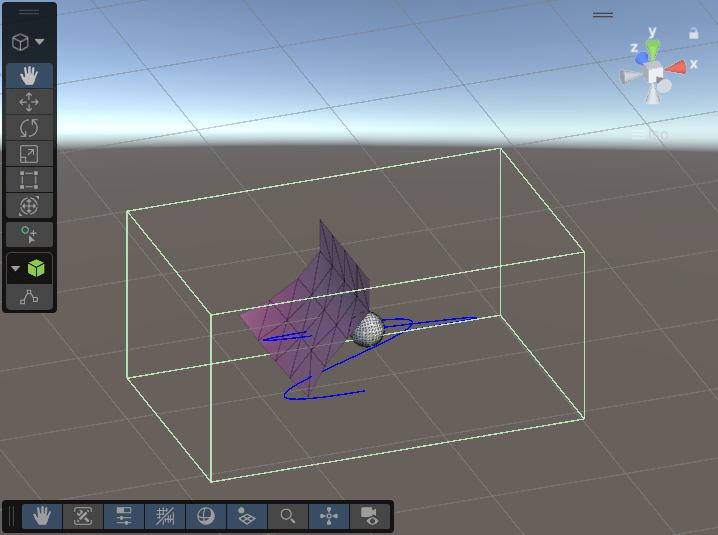
\includegraphics[width=0.5\textwidth]{Imagenes/Bmap/spline.png}
    \caption{Movimiento aleatorio basado en splines.}
    \label{fig:spline}
\end{figure}

El movimiento aleatorio es el empleado para generar datasets para lso experimentos y mayor parte del desarollo del proyecto, pues aporta mayor número de deformaciones e información de la tela, dando capacidad de generalización al modelo. La zona de generación de movimientos de la bola está ajustada de tal forma que se aumente el número de colisiones con la tela en el tiempo de la simulación sin realizar deformaciones exageradas.

\subsection{Otras simulaciones}
También cabe mencionar brevemente que durante el desarollo del proyecto se han realizado pruebas con simulaciones más complejas con objeto de probar la efectividad de nuestro método y diferencias entre simulaciones más dinámicas y estáticas, más frecuentadas en PBD. Realizar estas pruebas más complejas resultó incompatible con nuestra plataforma elegida y capacidad de cómputo. \newline 

Para probar el enfoque más estático y pegado al cuerpo se creó una simulación de un personaje con una camiseta. Tras múltiples pruebas tomando diferente número de iteraciones en el solver de Cloth, valores en las propiedades de la tela y extendido el tamaño hasta 4000 vértices, la simulación fue finalmente descartada debido a la inestabilidad de la tela y difícil generación de animaciones visualemente coherentes. Realizar animaciones de tela complejas en Unity sin combinar otras técnicas, implementar soluciones híbridas (como el Weight Mapping\footnote{Técnica de animación 3D y rigging que permite controlar cómo se deforman los vértices de una malla o prenda al mover las articulaciones de un esqueleto. }) o incorporar paquetes de pago de la Unity Asset Store como Magica Cloth \footnote{Paquete de Magica Cloth en el Asset Store de Unity:  \url{https://assetstore.unity.com/packages/tools/physics/magica-cloth-2-242307}} u Obi Cloth no es trivial. Otras investigaciones, como \cite{holden_subspace_2019} producen su material de entrenamiento en herramientas especializadas como Maya \footnote{Autodesk Maya es un software profesional de animación y efectos visuales 3D \url{https://www.autodesk.com/es/products/maya/overview}} o Blender \footnote{Blender es un software de código abierto de animación y efectos visuales 3D  \url{https://www.blender.org/}} para conseguir simulaciones de prendas complejas. Pese a que esto limita el alcance de las simulaciones a generar en esta investigación, el nivel de complejidad potencial sigue siendo más que sufiente para probar nuestra implementación a pequeña escala, manteniendo el proyecto alienado a los objetivos previamente declarado y siguiendo la tendencia de juegos implementados en Unity.  \newline 

\begin{figure}[H]
    \begin{minipage}{0.48\textwidth}
        \centering
        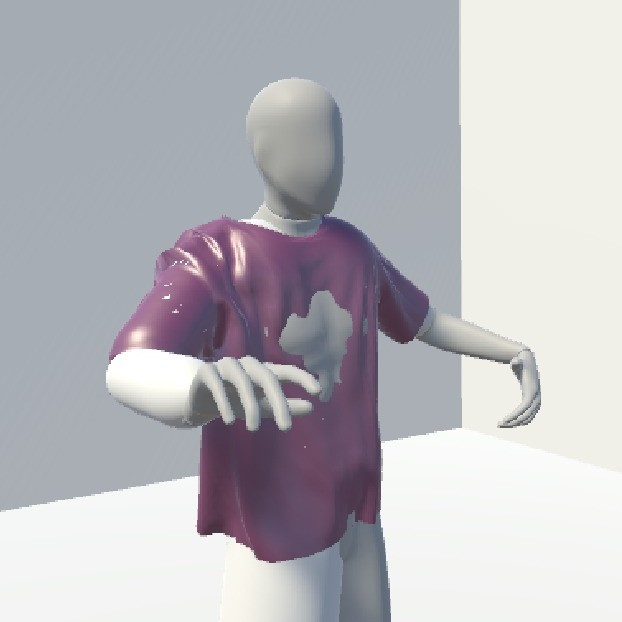
\includegraphics[width=0.8\textwidth]{Imagenes/Bmap/prubacamiseta.jpeg}
        \caption{Simulación de una camiseta con componente Cloth.}
        \label{fig:camiseta}
    \end{minipage}
    \hfill
    \begin{minipage}{0.48\textwidth}
        \centering
        
\includegraphics[width=0.8\textwidth]{Imagenes/Bmap/skirt.png}
        \caption{Simulación de una falda con componente Cloth.}
        \label{fig:skirt}
    \end{minipage}
\end{figure}

\begin{comment}
La otra simulación llevada a cabo consiste en un personaje andando con una \textbf{falda}. El personaje, simplificado, está formado por tres cápsulas: un torso y dos piernas; y la falda es un malla en forma de cilindro compuesta por 288 vértices, para habilitar un movimiento más dinámico. Una vez ajustados los colliders de las cápsulas para ser más grandes que las mallas de las piernas, esta simulación genera un buen resultado a nivel visual. Lo emplearemos más adelante para representar animaciones más complejas y realizar  comparaciones y mediciones adicionales al plano de 25 vértices.
\begin{figure}[htbp]
    \centering
    
\includegraphics[width=0.6\textwidth]{Imagenes/Bmap/skirt.png}
    \caption{Simulación de una falda con componente Cloth.}
    \label{fig:skirt}
\end{figure}
\end{comment}

\subsection{Los parámetros}
Las telas que usamos para generar las simulaciones en las que se basan nuestros modelos son objetos formados por mallas con un componente Cloth (y su correspondiente \textit{Skinned Mesh Renderer}) y un componente de grabación propio \textit{ClothDatasetRecorder}, encargado de guardar los datos de la simulación. Se plantea recoger diferentes parámetros que representen las características más importantes de la tela durante la simulación:  \newline

\begin{itemize}
    \item \textbf{Posición}: Las posiciones de los vértices de la tela son los parámetros básicos de las investigaciones en este campo.
    \item \textbf{SDF}: El Signed Distance Field es una magnitud que representa la distancia de cada vértice al objeto colisionador, llegando a ser 0 si toca la superfície, y un valor negativo si alcanza a traspasar. Se ha creado la clase estática \textit{SDFUtil} para habilitar los cálculos del SDF para conjuntos de \textit{colliders} en escenarios más complejos. El script \textit{SDFUtil} contiene métodos que proporcionan el SDF de un punto a una esfera, una cápsula o dos listas de los dos tipos. También acepta un \textit{Transform} de un objeto de referencia si la posición del punto de origen no es global.

    Las fórmulas de SDF, así como la obtención de un único SDF respecto a varios objetos, que se ha decidido representar con el \textit{Smooth Mininum} (\textit{smin}), se han adquirido del blog de Inigo Quilez\footnote{Apartado del blog de Inigo Quilez sobre SDFs para objetos 3Ds: \url{https://iquilezles.org/articles/distfunctions/}} y adaptado para el funcionamiento esperado en Unity. La función \textit{smin} permite fusionar dos objetos de geométricamente con una transición que puede ser suave o limitarse al espacio real ocupado por los objetos.

    \item \textbf{Velocidad}: Planteamos que las velocidades de los vértices pueden ayudar a que el modelo sea capaz de replicar el dinamismo del movimiento. 
    \item \textbf{Normales}: Refiriéndose a las normales de la superficie del objeto colisionador, es decir, el gradiente del SDF. Este se puede usar para complementar la magnitud del SDF, ya que apunta en la dirección en la que la distancia aumenta más rápido, cómo alejarse de la colisión.
    \item \textbf{UVs}: Conservar la geometría de la tela se plantea como uno de los mayores retos para nuestra simulación. Se necesita que el modelo comprenda cómo están relacionados los vértices espacialmente para que no se lleven a cabo deformaciones érroneas. Ya que no comenzamos con geometrías complejas en tela o cuerpos blandos, se usan las coordenadas de textura bidimensionales, \textit{UVs}, para representar la superfície.
    \item \textbf{Máxima Distancia}: Cada vértice tiene una distancia máxima a la que un vértice se puede mover desde su posición en la malla \textit{skinned}\footnote{Una \textit{skinned mesh} es una malla poligonal 3D cuyos vértices están unidos a un esqueleto jerárquico de huesos, que permite la deformación dinámica de sus vértices.}. Se quiere conseguir que los vértices no se pasen de su rango hábil de movimiento. Si no se toma como parámetro, esto puede corregirse también en post-procesamiento.
\end{itemize}

\subsubsection{Sistema de coordenadas}
Cabe recalcar que el registro de las posiciones se realiza de forma local respecto al pivote de la tela. Pese a que tanto utilizando posiciones globales (reales en el mundo) como locales se mantiene la consistencia y un origen único de coordenadas, las posiciones locales son más relevantes para los modelos y los resultados no son dependientes de las traslaciones en el espacio. Se ha confirmado la relevancia de emplear un \textbf{sistema de coordenadas local} tras evaluar el desempeño del modelo con datasets relativos a ambos sistemas.

En Cloth, las posiciones de los vértices de la tela ya se obtienen de forma relativa a su pivote. Unity proporciona los métodos \textit{TransformPoint(Vector3 position)} y \textit{InverseTransformPoint(Vector3 position)} para obtener coordenadas de mundo a partir de coordenadas locales de un objeto y para pasarlas a coordenadas locales a partir de un transform respectivamente. Se utilizan estos métodos para realizar todos los cálculos y proporcionar al modelo los datos en en el mismo sistema de coordenadas. \newline

\subsubsection{Elección de parámetros finales}
Ante la gran cantidad de datos recogidos, se investigan maneras de seleccionar las características más esenciales para el entrenamiento. Tras confirmar con estudios como \cite{chen2020selecting} o \cite{iranzad2025review} que el uso de modelos \textit{Random Forest} para la reducción de features puede ser interesante, se implementa uno de estos modelos para ver cuáles son los parámetros más importantes para la inferencia. Se mide la importancia de Gini, esta métrica mide la reducción media de la impureza (MDI por sus siglas en inglés: Mean Decrease in Impurity), es decir, cuánta varianza o error reduce cada variable a lo largo de las divisiones en los nodos de todos los árboles. Sumando la importancia acumulada sobre los ejes temporales y espaciales (vértices de la malla), se consigue obtener la importancia de cada una de las 13 propiedades del dataset. Como se ve en la figura, los parámetros U, V y MD resultan no ser importantes para generar la predicción. Sin embargo, se aprecia la importancia de los parámetros de velocidad. En este caso es más notable en el eje x, debido a la configuración de la simulación con la que se ha generado el dataset analizado para el gráfico (\ref{fig:random_forest}).
\begin{figure}[H]
    \centering
    
\includegraphics[width=0.6\textwidth]{Imagenes/resultRndFrst.png}
    \caption{Parámetros valorados por el random forest.}
    \label{fig:random_forest}
\end{figure}


\subsection{Generación del dataset}
A través del componente \textit{ClothDatasetRecorder} realizamos un ``snapshot'' o captura de la tela cada intervalo de tiempo \textit{recordTime}, que se declara en el inicio del desarollo como 3.5 segundos. Estos datos del frame se guardan en una estructura SnapInfo, que representa la información de los vértices de la tela en un instante de tiempo determinado, y se añade a una lista de capturas de la simulación. 
Al final de la ejecución todas estas capturas se transforman en texto y se vuelcan en un CSV, por lo que cada línea del archivo corresponde a un frame capturado. \newline


\begin{algorithm}[H]
\caption{Struct SnapInfo: representación de un frame}
\SetKwData{SnapInfo}{SnapInfo}
\SetKwComment{Comment}{$\triangleright$\ }{}

\KwData{
  \SnapInfo\ \{\\
  \quad $\mathbf{pos}$: array de Vector3 \Comment*[r]{posiciones}\\
  \quad $\mathbf{vel}$: array de Vector3 \Comment*[r]{velocidades}\\
  \quad $\mathbf{normal}$: array de Vector3 \Comment*[r]{normales}\\
  \quad $\mathbf{sdf}$: array de float \Comment*[r]{signed distance field}\\
  \quad $\mathbf{maxDist}$: array de float \Comment*[r]{distancia máxima}\\
  \quad $\mathbf{uv}$: array de Vector2 \Comment*[r]{coordenadas UV}\\
  \}
}
\end{algorithm}

Durante el inicio del estudio se probaron distintas frecuencias de muestreo (0.1f, 0.02f, la frecuencia por defecto del \textit{FixedUpdate()} en Unity); pero más tarde se llegaría a la conclusión de que la frecuencia de muestreo debe ser la misma en la etapa de guardado de datos y ejecución del modelo. De la misma forma, el número de snapshots debe ser el máximo posible para garantizar la estabilidad de la simulación. Al tratarse de una simulación con inercia y no basada en poses, la frecuencia no admite reducciones.